\documentclass[a4paper, 12pt, onepage]{article}
\usepackage{graphicx}
\usepackage{lipsum}
\usepackage{mathptmx}


\usepackage{fancyhdr}
\pagestyle{fancy}
\fancyhead{}
\fancyfoot{}
\fancyhead[R]{\thepage\ \hspace{1pt} }

\renewcommand{\headrulewidth}{0pt}
\renewcommand{\footrulewidth}{0pt}

\begin{document}
\pagenumbering{roman}
\addcontentsline{toc}{section}{Title Page}
\begin{titlepage}
  \centering
  
\includegraphics[width=0.2\textwidth]{tu_logo.png}\par
  {\large\scshape Tribhuvan University\par}
  \vspace{0.3cm}
  {\large Pulchowk, Lalitpur \par}
  \vspace{3cm}
  	{\large\scshape A\par}
	{\large\scshape Major Project\par}
        {\large\scshape On\par}
        {\large\scshape Personality Based Music Recommendation System\par}
	\vspace{2.5cm}
        {\large\scshape Submitted by:}\\
        \vspace{0.2cm}
        {
          {\normalsize\verb+Nabin Bhattarai(070/BCT/522)+}\\
          \vspace{0.1cm}
          {\normalsize\verb+Miran Ghimire(070/BCT/521)+}\\
          \vspace{0.1cm}
          {\normalsize\verb+Brihat Ratna Bajracharya(070/BCT/513)+}\\
          \vspace{0.1cm}
          {\normalsize\verb+Abhishek Paudel(070/BCT/502)+}\\
          \vspace{0.1cm}
        }
        \vspace{1cm}
        {\large\scshape Supervised By}\\
        \vspace{0.2cm}
        {
          {\normalsize \verb+Daya Sagar Baral+\par}
          \vspace{0.1cm}
          {\normalsize \verb+Department of+\par}
          \vspace{0.1cm}
          {\normalsize\verb+Electronics and Computer Engineering+}
          \vspace{0.1cm}
        }
        
        \vspace{1cm}
        \vfill

        % Bottom of the page
	{\normalsize \today\par}
      \end{titlepage}

      \setcounter{page}{2}
      \cleardoublepage
      {
        \setlength{\parskip}{0em}
        \renewcommand\contentsname{Table of Contents}
        \tableofcontents \addcontentsline{toc}{section}{Table of Contents}
      }


      \cleardoublepage
      \pagenumbering{arabic}
      \section{Introduction}
	``\textbf{Personality Based Music Recommendation}'' is the system which uses social media profile of a person to recommend the appropriate music to that user. In this contemporary era of digital technologies, social media has become one of the prominent means for information sharing and communication. Likewise music has been one of the prominent market of entertainment. People listen to music everyday. The fact that music can blend with any emotion has made it's way to different sorts of people with different sorts of personality.\\
	Hence we have come up with the system to recommend the music to a different people based on their social media profiles.Previous work has shown that the information in users social media profiles is reflective of their actual personalities, not an idealized version of themselves, which makes social media platform for studying a people personality.\\
	Several well studied personality models have been proposed, among which the Big Five model is established as the most popular one,which suggests that the regularity in someone's behavior over time and situations uniquely identifies his/her personality type along five dimesions: Openness to experience, Neuroticsm, Extroversion, Aggreableness and Conscientiousness.

      \cleardoublepage
      \section{Summary Of Process}
      \begin{figure}[ht!]
	      \includegraphics[width=450px]{pbrs.png}
		\caption{Block Diagram of a System}
	\end{figure}
	\subsection{Task Analysis}
	\begin{center}
		\begin{tabular}{|c|l|c|c|}
			\hline
				Activity & Description & Immediate Predecessors&Time(weeks)\\
			\hline
			A&Personality DataSet Analysis&-&1\\
			\hline
			B&Feature Extraction from Personality DataSet&A&3\\
			\hline
			C&Personality Analysis Model&B&4\\
			\hline
			D&User Social Media Information Extraction&-&1\\
			\hline
			E&User Personality Analysis&D,C&2\\
			\hline
			F&Music DataSet Analaysis&-&1 \\
			\hline
			G&Feature Extraction from Music DataSet&F&2\\
			\hline
			H&Recommendation Model&G,E&4\\
			\hline
			I&Testing and Debugging&H&2\\
			\hline

		\end{tabular}
	\end{center}
	\cleardoublepage
	\subsection{Task Evaluation}
		\subsubsection{Task Completed}
		\begin{enumerate}
		\item Personality DataSet Analysis
		\item Feature Extraction from Personality DataSet
		\item Personality Analysis Model
		\end{enumerate}

		\subsubsection{Task Remaining}
		\begin{enumerate}
		\item User Social Media Information Extraction
		\item User Personality Analysis
		\item Music DataSet Analysis
		\item Feature Extraction from Music DataSet
		\item Recommendation Model
		\item Testing and Debugging
		\end{enumerate}
      \subsection{Schedule Analysis}
      \begin{figure}[ht!]
	      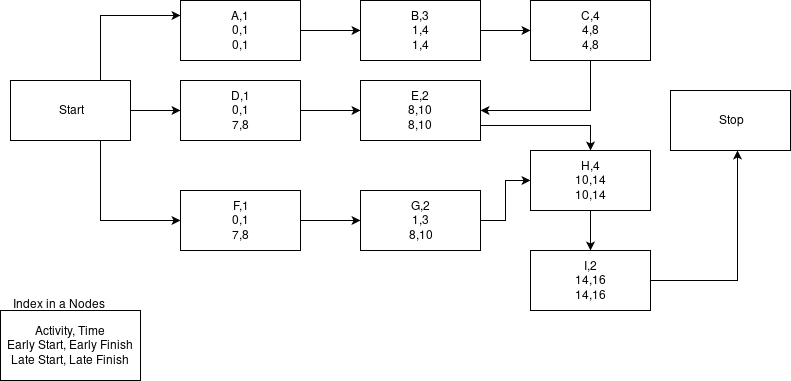
\includegraphics[width=450px]{aschedule.png}
	      \caption{Activity of Node Diagram of Project}
	\end{figure}
      \subsection{Budget Analysis}
      \subsection{Scope Analysis}
      \subsection{Process Analysis}
      \subsection{Gantt Progress Chart}

      \cleardoublepage
      \section{Activity Analysis}
      \subsection{Task completed since last report}
      \subsection{Current tasks and deliverable}
      \subsection{Short term future tasks and deliverable}

      \cleardoublepage
      \section{Previous problems and issues}
      \subsection{Action item and status} %k vanya maile bujhena hai
      \subsection{New or revised action items} %yo ni

      \cleardoublepage
      \section{New problems and issues}
      \subsection{Problems}
      \subsection{Issues}
      \subsection{Possible solutions}
      \subsubsection{Recommendation}
      \subsubsection{Assignment of responsibility}
      \subsubsection{Deadline}
\end{document}

%%% Local Variables:
%%% mode: latex
%%% TeX-master: t
%%% End:
